\documentclass{beamer}
\usetheme{Boadilla}
\usecolortheme{dolphin}
\setbeamertemplate{navigation symbols}{}

\usepackage[utf8]{inputenc}
\usepackage[T1]{fontenc}
\usepackage[polish]{babel}
\usepackage{hyperref}
\usepackage{graphicx}
\usepackage{booktabs}
\usepackage{xcolor}
\usepackage{amsmath}

\newtheorem{thm}{Twierdzenie}
\newtheorem{df}{Definicja}

\title{Jak wygląda modelowanie matematyczne}
\subtitle{czyli czy opłaca się biegać w deszczu?}
\author{Vlad Snozyk}
\institute{Wydział Matematyki i Informatyki UJ}
\date{\today}

\begin{document}

\begin{frame}
  \titlepage
\end{frame}

\begin{frame}{Model matematyczny na studiach}
  Przykłady świetnych modeli matematycznych:
  \begin{itemize}
    \item Wyznacznik
    \item Liczby zespolone
    \item Pochodne
  \end{itemize}
\end{frame}

\begin{frame}{Model matematyczny na studiach}
  Teoria teorią, ale w praktyce jest troszczkę inaczej\ldots
\end{frame}

\begin{frame}{Problem biegania pod deszczem}
  Na ulicy stoi człowiek. Nagle zaczyna padać deszcz. Osoba kieruje się do
  najbliższego schronienia oddalonego o $l$ metrów.

  \vspace{0.5cm}
  \textbf{Pytanie:} jaką prędkością powinien się poruszać, aby zmoknąć jak najmniej?
\end{frame}

\begin{frame}{Problem biegania pod deszczem — formalizacja}
  Prostopadłościan o powierzchniach $a$, $b$, $c$ porusza się z prędkością
  prostopadłą do powierzchni $a$. Pada deszcz, gdzie:
  \begin{itemize}
    \item każda kropla ma prędkość $v$
    \item ilość kropli w jednostce objętości wynosi $k$
  \end{itemize}

  \vspace{0.4cm}
  \textbf{Pytania:}
  \begin{itemize}
    \item Ile kropli $N$ trafi w prostopadłościan podczas przemieszczenia o $l$?
    \item Przy jakiej prędkości $N$ jest minimalne?
  \end{itemize}
\end{frame}

\begin{frame}{Rozwiązanie — krok 1}
  \begin{block}{Uproszczenie}
    Olewamy boczną stronę i przechodzimy do uproszczonego problemu 2D.
  \end{block}
\end{frame}

\begin{frame}{Problem uproszczony}
  Na prostopadłościan pada deszcz z prędkością $v$ przez czas $t$ sekund.
  Ilość kropli w jednostce objętości wynosi $k$.

  \vspace{0.4cm}
  \textbf{Pytanie:} ile kropli trafi w prostopadłościan?

  \vspace{0.4cm}
  $$\vec{v} = \vec{v_x} + \vec{v_y}$$
\end{frame}

\begin{frame}{Plots}
  \begin{figure}
    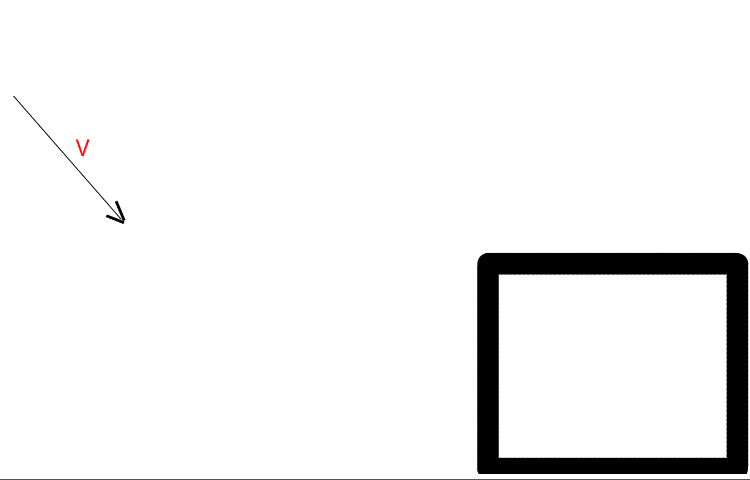
\includegraphics[width=\textwidth]{pt1.png}
  \end{figure}
\end{frame}

\begin{frame}{Plots}
  \begin{figure}
    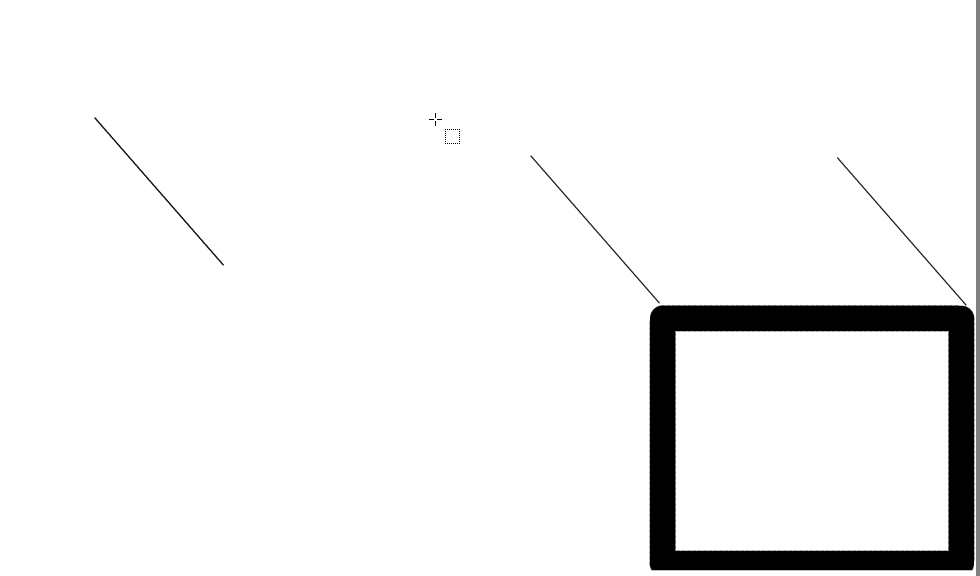
\includegraphics[width=\textwidth]{pt2.png}
  \end{figure}
\end{frame}

\begin{frame}{Plots}
  \begin{figure}
    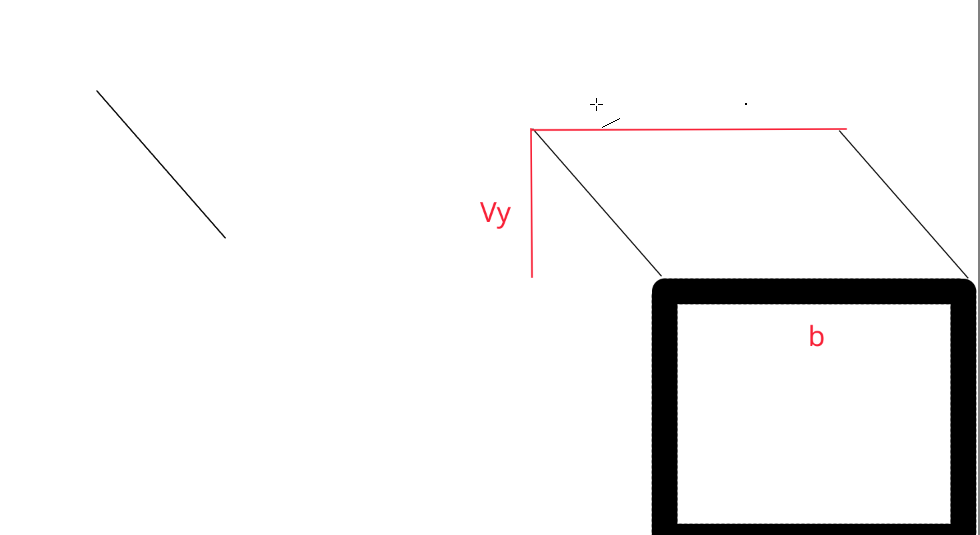
\includegraphics[width=\textwidth]{pt3.png}
  \end{figure}
\end{frame}

\begin{frame}{Plots}
  \begin{figure}
    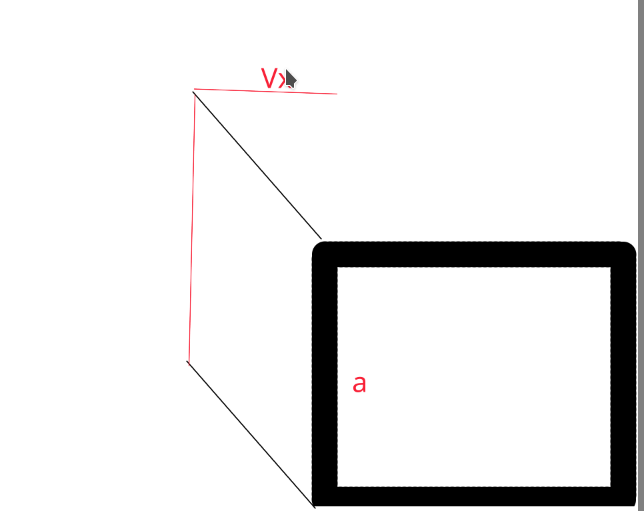
\includegraphics[width=200pt]{pt4.png}
  \end{figure}
\end{frame}

\begin{frame}{Wzór}
  $$\text{Volume} = (V_x \cdot a + V_y \cdot b) \cdot t$$
  $$N = \text{Volume} \cdot k = (V_x \cdot a + V_y \cdot b) \cdot t \cdot k$$
\end{frame}

\begin{frame}{Wzór ogólny}
  $$N = (V_x \cdot a + V_y \cdot b + V_z \cdot c) \cdot t \cdot k$$
\end{frame}

\begin{frame}{Ruch względny}
  Przykłady ruchu względnego:
  \begin{itemize}
    \item Słońce
    \item Ziemia
    \item Pociąg
    \item \href{https://www.youtube.com/watch?v=8wqNX7_4vAE}{Filmik z pieskiem}
  \end{itemize}
\end{frame}

\begin{frame}{Animacje}
  Animacje ilustrujące ruch względny i problem deszczu.
\end{frame}

% ── Przypadek 1 ───────────────────────────────────────────────────────────────

\begin{frame}{Przypadek 1 — wiatr wieje w twarz}
  \begin{block}{Ustawienie}
    Wiatr wieje przeciwnie do kierunku ruchu człowieka.
  \end{block}
\end{frame}

\begin{frame}{Przypadek 1 — wiatr wieje w twarz}
  \begin{align*}
    t &= \frac{l}{u} \\
    V_x^* &= V_x + u
  \end{align*}
\end{frame}

\begin{frame}{Przypadek 1 — wiatr wieje w twarz}
  \begin{align*}
    t &= \frac{l}{u}, \quad V_x^* = V_x + u \\[6pt]
    N &= (V_x^* \cdot a + V_y \cdot b + V_z \cdot c) \cdot t \cdot k \\[6pt]
    N(u) &= \frac{(V_x + u) \cdot a + V_y \cdot b + V_z \cdot c}{u} \cdot l \cdot k
  \end{align*}
\end{frame}

\begin{frame}{Przypadek 1 — wiatr wieje w twarz}
  \begin{align*}
    N(u) &= \frac{(V_x + u) \cdot a + V_y \cdot b + V_z \cdot c}{u} \cdot l \cdot k \\[6pt]
    N(u) &= \frac{V_x \cdot a + V_y \cdot b + V_z \cdot c}{u} \cdot l \cdot k \;+\; a \cdot l \cdot k
  \end{align*}

  \vspace{0.3cm}
  \begin{block}{Wniosek}
    Im większa prędkość $u$, tym mniejsza liczba kropli — biec jak najszybciej.
  \end{block}
\end{frame}

\begin{frame}{Plots}
  \begin{figure}
    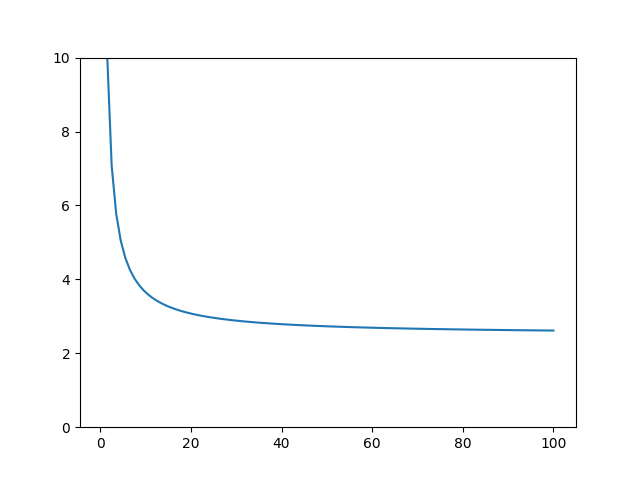
\includegraphics[width=250pt]{pt5.png}
  \end{figure}
\end{frame}

% ── Przypadek 2 ───────────────────────────────────────────────────────────────

\begin{frame}{Przypadek 2 — wiatr wieje w plecy}
  \begin{block}{Ustawienie}
    Wiatr wieje w tym samym kierunku co ruch człowieka.
  \end{block}
\end{frame}

\begin{frame}{Przypadek 2 — wiatr wieje w plecy}
  Animacje.
\end{frame}

\begin{frame}{Przypadek 2 — wiatr wieje w plecy}
  \begin{align*}
    t &= \frac{l}{u} \\
    V_x^* &= V_x - u
  \end{align*}
\end{frame}

\begin{frame}{Przypadek 2 — wiatr wieje w plecy}
  \begin{align*}
    t &= \frac{l}{u}, \quad V_x^* = V_x - u \\[6pt]
    N &= (V_x^* \cdot a + V_y \cdot b + V_z \cdot c) \cdot t \cdot k \\[6pt]
    N(u) &= \frac{|V_x - u| \cdot a + V_y \cdot b + V_z \cdot c}{u} \cdot l \cdot k
  \end{align*}
\end{frame}

\begin{frame}{Przypadek 2 — podprzypadki}
  \textbf{Gdy $V_x > u$:}
  \begin{align*}
    N(u) &= \frac{V_x \cdot a + V_y \cdot b + V_z \cdot c}{u} \cdot l \cdot k \;-\; a \cdot l \cdot k
  \end{align*}

  \vspace{0.2cm}
  \textbf{Gdy $V_x \leq u$:}
  \begin{align*}
    N(u) &= \frac{-V_x \cdot a + V_y \cdot b + V_z \cdot c}{u} \cdot l \cdot k \;+\; a \cdot l \cdot k
  \end{align*}

  \vspace{0.2cm}
  \begin{block}{Wniosek}
    W obu przypadkach im większa prędkość, tym mniej kropli — biec jak najszybciej.
  \end{block}
\end{frame}

\begin{frame}{Plots}
  \begin{figure}
    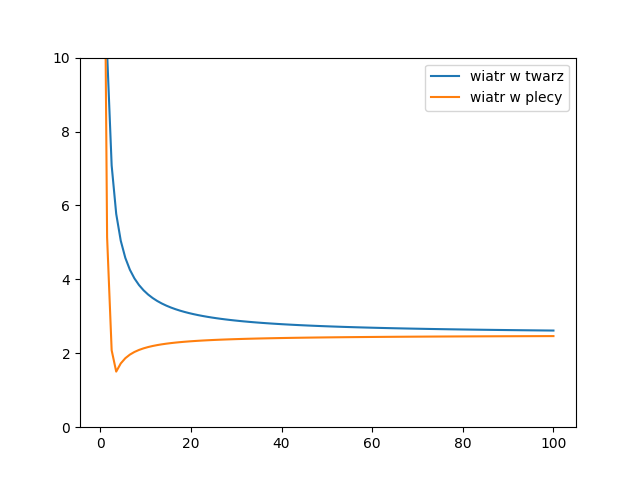
\includegraphics[width=250pt]{pt6.png}
  \end{figure}
\end{frame}

\begin{frame}{Pytania}
  \centering
  \Large
  Czy są jakieś pytania?
\end{frame}

\end{document}
